% Build from manuscript/ so the figure and bibliography resolve locally.
% From the project root: latexmk -cd -pdf manuscript/main.tex
\documentclass[12pt]{article}
\usepackage{graphicx}
\usepackage{setspace}
\usepackage{geometry}
\usepackage{natbib}
\usepackage{times}
\usepackage{hyperref}
\usepackage{amsmath}
\usepackage{amsfonts}
\usepackage{amssymb}

\geometry{margin=1in}
\doublespacing

\title{Foreign Investor Rights in Pakistan's Energy Sector: Does Chinese Sponsorship Reduce Renegotiation Risk?}
\author{Andrew Wang, Hassan Aziz}
\date{Dec 2025}

\begin{document}
\maketitle

\section{Introduction}
The political economy of foreign investment in states with weak institutions presents a fundamental puzzle: how do governments credibly commit to honoring investor rights when institutional guarantees, such as independent judiciaries or constitutional checks, are absent or unreliable? Despite these limitations, countries with weak institutions have to and, in some cases, manage to attract foreign investment, specifically in strategic sectors such as energy. How do countries with weak institutions that attract significant amounts of investment manage to do so? This question becomes even more puzzling when such investments persist under conditions of fiscal crisis, political instability, and public dissent.

This paper explores this puzzle through the lens of Pakistan’s Independent Power Producers (IPPs), with a particular focus on Chinese firms operating under the China-Pakistan Economic Corridor (CPEC). These IPPs (mostly owned by private Chinese companies) have made significant investments in Pakistan’s energy sector, on the promise of government guaranteed long-term Power Purchase Agreements (referred to as PPAs, hereafter) that include generous dollar-denominated returns. These generous returns have faced significant criticism and calls for reform due to escalating associated debt, however, successive Pakistani governments have failed to revise or terminate these contracts despite the absence of institutional arrangements preventing it to do so \citep{BusinessRecorder2024a}.

To investigate why Pakistan’s state has been unable to renegotiate the PPAs, this paper develops a formal theory of political commitment under institutional weakness and applies it to the case of Pakistan. It introduces the concept of Vertical Political Integration (VPI) to explain how political coalitions that span domestic and international actors can sustain investment relationships without formal enforcement mechanisms. Drawing on this framework, the paper tests whether Chinese-owned IPPs are more insulated from renegotiation than non-Chinese counterparts, especially following economic or political shocks. As this is the first draft of this paper, the empirical analysis section is underdeveloped, however, it will be based on original data on IPP ownership, contract terms, plant performance, and renegotiation attempts.

\section{Puzzle}
The paradox of Pakistan’s power sector lies in the coexistence of surplus generation capacity and persistent blackouts, escalating tariffs, and fiscal burden. According to the Economic Survey (2023--24), Pakistan’s installed electricity generation capacity reached 42{,}131 MW, almost twice the average domestic demand \citep{PakistanSurvey2024}. However, the electricity tariffs have risen sharply in the last few years. A \textit{Bloomberg} report noted in some residential areas, the cost of powering a home exceeds that of renting one, driven by sharp tariff hikes required to fulfill IMF bailout conditionalities\footnote{The IMF packages have repeatedly asked the government to rationalize the cost of electricity by charging consumers a price equal to the total production cost and remove subsidies that force the government to increase borrowing, causing hikes in inflation and interest rate and damaging economic growth.} \citep{Kiani2024}. This seeming contradiction---abundance coexisting with high costs---has fueled criticism of Independent Power Producers (IPPs), including those affiliated with China’s Belt and Road Initiative under the China-Pakistan Economic Corridor (CPEC).

The source of this fiscal and distributional dysfunction lies in the structure of Power Purchase Agreements (PPAs), which guarantee capacity payments to IPPs irrespective of electricity demand. Many of these contracts offer dollar-indexed returns on equity ranging from 27--34\%, far surpassing the 15--18\% returns under Pakistan’s 1994 energy policy \citep{IEEFA2020}. These high rents are guaranteed even when plants operate below capacity or remain idle, contributing to circular debt in the power sector and driving electricity costs to unsustainable levels. Despite mounting public pressure and statements by public figures, renegotiation of contracts has taken place only with local firms and no major renegotiations have taken place with the Chinese-firm-owned IPPs \citep{BusinessRecorder2024b}.

Historically, Pakistan’s energy sector was liberalized through the landmark 1994 Energy Policy, which, backed by the World Bank, attracted \$6.5 billion in investment and added 6{,}500 MW to the grid. However, by 1998, the government struggled to fulfill contractual obligations, and by 2013, energy deficits had returned. CPEC, initiated in 2014, allocated over \$35 billion to the power sector. Though this added over 6{,}000 MW through coal-fired projects, it also entrenched Pakistan in a web of high-cost contracts with Chinese and local energy-producing firms.

\section{Research Questions}
The puzzle is: Why does Pakistan, despite public opposition\footnote{Elections provide a threat to the government of being ousted and give credibility to public opposition. Elections are an important part of the puzzle as power outages and prices have been at the heart of electoral politics in the last decade \citep{Ravi2023}.} and repeated fiscal crises and in the absence of strong legal institutional structures, fail to restructure or exit the costly contracts with Chinese-owned IPPs? From this paradox, the empirically tractable research question is:

\begin{quote}
\textit{Do Chinese-owned IPPs under CPEC receive fewer attempts at contract revision or tariff reduction compared to non-Chinese IPPs, following fiscal or political shocks?}
\end{quote}

\section{Brief Literature Review}
\textit{Note: I have kept the literature review focused on the theory and not detailed the literature focused on energy politics, the role of trade in geopolitics, and literature focusing on Chinese international investments.}

Foundational models in the political economy of investment and institutional development underscore the need for commitment mechanisms in environments of uncertainty. Olson \citeyearpar{Olson1993} posits that rulers with long time horizons may refrain from predation to ensure long-term revenue through investment growth. Similarly, North and Weingast \citeyearpar{NorthWeingast1989} emphasize how institutional checks and legal frameworks constrain rulers, creating credible commitments that facilitate private investment. These insights remain influential in understanding political order and economic development.

However, in fragile or transitional states like Pakistan, where institutions are weak, time horizons short, and authority dispersed, formal institutional constraints may be inadequate or absent. Here, the mechanisms described above may become less predictive. In such settings, a different logic of enforcement may be operative, one that relies on informal, political arrangements rather than impersonal legal mechanisms. The most compelling theoretical alternative in such contexts is the framework of Vertical Political Integration (VPI), introduced in the book \textit{The Politics of Property Rights} \citep{Haber2003}. VPI explains how credible commitments can emerge through politically structured, vertically integrated coalitions between states, investors, and third-party enforcement agents. Under VPI, property rights are not universally enforced public goods but selectively applied privileges allocated to those within the ruling coalition.

\section{Theory}
Vertical Political Integration \citep{Haber2003} is a governance system in which a state facing institutional fragility and political instability sustains investment and property rights through selective enforcement and informal coalitional arrangements. In a VPI system, the state does not treat all investors equally. Instead, it privileges certain actors (i.e., actors that are embedded in the political elite or linked to strategic interests) with monopolistic guarantees and protection from expropriation. In return, these asset holders provide economic resources, political support, and often technical or logistical services that bolster the state’s authority.

Building on the extended theory of VPI, three foundational conditions enable such systems to function. First, property rights are enforced as private goods rather than public goods. This enforcement is selective, targeting only those actors who are integrated into the governing coalition. Second, VPI systems require the formation of rent-sharing coalitions among governments, asset holders, and third-party enforcers. These coalitions generate, distribute, and protect rents in exchange for political loyalty and investment commitment. Third, enforcement mechanisms are informal, contingent, and often ad hoc---relying on reputational pressure, the threat of sanction, or diplomatic leverage rather than codified legal norms.

The empirical case of CPEC IPPs in Pakistan exemplifies this logic. Pakistan’s public institutions are too weak to uniformly enforce contract renegotiation or accountability. Yet, Chinese IPPs continue to enjoy exceptional protection. Their status stems from their integration not just into Pakistan’s regulatory system, but into its political economy via elite alignment and geopolitical strategy. These firms are tied to state-backed Chinese capital and embedded within a wider BRI framework. The Chinese state acts as the third-party enforcer, using leverage to deter any Pakistani deviation. As a result, CPEC energy deals persist despite intense domestic opposition, deep fiscal burdens, and technical underperformance.

Unlike theoretical models that assume universal enforcement, VPI recognizes that political survival in weak states often hinges on maintaining targeted investor coalitions. The high returns, capacity payments, and privileged billing practices enjoyed by Chinese firms are not merely legacy features of old contracts but are actively maintained by an informal, vertically integrated political coalition. These dynamics explain how economic inefficiency can persist as a rational political equilibrium.

\section{Formal Model}

We develop a continuous-time model of government–IPP relations consistent with our empirical strategy, which estimates whether Chinese-owned Independent Power Producers (IPPs) exhibit a systematically lower hazard of renegotiation than non-Chinese IPPs. The theoretical framework draws on Vertical Political Integration (VPI), which posits that politically integrated foreign investors receive selective enforcement of property rights backed by external actors.

Consider a set of IPPs indexed by $i = 1,\dots,N$. Let $T_i$ denote the random time until the first renegotiation attempt targeting IPP $i$'s Power Purchase Agreement (PPA). The government faces recurrent political and fiscal pressures that may motivate renegotiation, but renegotiation also entails diplomatic, financial, and reputational costs. 

At each instant $t$, the government evaluates the net benefit of initiating renegotiation of IPP $i$:
\[
\Delta U_i(t) = B_i(t) - C_i(t) + \nu_i(t),
\]
where $B_i(t)$ captures political or fiscal benefits of renegotiation, $C_i(t)$ represents associated costs, and $\nu_i(t)$ is an idiosyncratic shock.

\subsection*{Selective Enforcement Under VPI}

For non-Chinese IPPs, costs of renegotiation are primarily domestic or administrative. For Chinese IPPs, however, VPI implies the existence of an external enforcement agent (the Chinese state), which raises the expected diplomatic or financial cost of renegotiation. Let $\alpha_i$ indicate political integration:
\[
\alpha_i = 
\begin{cases}
1 & \text{if IPP } i \text{ is Chinese-owned},\\
0 & \text{otherwise}.
\end{cases}
\]

Then the cost function can be written as
\[
C_i(t) = C_0 + \alpha_i P,
\]
where $P > 0$ represents the expected penalty or loss of future support imposed by the external enforcer in the event of renegotiation. Thus, Chinese IPPs ($\alpha_i = 1$) face systematically higher renegotiation costs.

IPP capacity $K_i$ also influences the costs and benefits of renegotiation: large plants are more prominent, more difficult to modify, and potentially more politically consequential. We therefore write the political benefit term as
\[
B_i(t) = \beta_0\alpha_i + \beta_1 K_i.
\]

Renegotiation occurs at the first instant in which $\Delta U_i(t)$ crosses a threshold. If $\nu_i(t)$ follows a Type I extreme value distribution, the probability of renegotiation in the next instant, conditional on no prior renegotiation, yields a proportional hazards structure:
\[
\lambda_i(t \mid X_i) = \lambda_0(t)\exp\left(\theta_1 \alpha_i + \theta_2 K_i \right),
\]
where $\lambda_0(t)$ is an unspecified baseline hazard and $X_i = (\alpha_i, K_i)$.

\subsection*{Implications}

VPI predicts that the international penalty $P$ depresses the renegotiation hazard for Chinese-owned IPPs. Since $\alpha_i$ directly parameterizes integration into the VPI coalition, the model implies:
\[
\theta_1 < 0.
\]
The coefficient $\theta_2$ reflects the independent effect of capacity on renegotiation risk.

The empirical strategy therefore estimates whether the hazard of renegotiation is systematically lower for Chinese IPPs, controlling for capacity, exactly as the theory implies.

\subsection{Interaction terms and Renegotiation After Fiscal Shocks}

One will notice, however, that most renegotiation events happen after some external fiscal shock. We now reframe the logic of Vertical Political Integration (VPI) in this setting.

The government observes a stream of shocks and political pressures over time and can, at any instant, initiate renegotiation. If no renegotiation has occurred by time $t$, the \emph{hazard rate} of renegotiation is defined as
\[
  \lambda_i(t) 
  = \lim_{\Delta t \to 0} 
    \frac{\Pr\big( t \leq T_i < t + \Delta t \,\big|\, T_i \geq t, X_i(t) \big)}{\Delta t},
\]
where $X_i(t)$ summarizes the political and economic conditions relevant to IPP $i$ at time $t$.

\subsection*{Government Payoffs and Renegotiation Incentives}

At each instant $t$, the host government $G$ faces a choice between maintaining the status quo or initiating a renegotiation of IPP $i$'s contract. The instantaneous net benefit to the government from initiating renegotiation at time $t$ can be written as
\[
  \Delta U_i(t) 
  = B^{\text{dom}}_i(t) - C^{\text{intl}}_i(t) - C^{\text{impl}}_i(t) + \nu_i(t),
\]
where:
\begin{itemize}
  \item $B^{\text{dom}}_i(t)$ is the domestic political benefit from attempting to revise the contract (e.g., signaling responsiveness to public anger over tariffs, demonstrating toughness vis-à-vis ``rent-seeking'' IPPs).
  \item $C^{\text{intl}}_i(t)$ is the expected international cost of targeting IPP $i$ (e.g., sanctions, loss of future financing, diplomatic fallout).
  \item $C^{\text{impl}}_i(t)$ is the implementation cost of renegotiation (legal, administrative, and technical constraints).
  \item $\nu_i(t)$ is an idiosyncratic shock to the perceived net benefit, capturing unobserved political or informational factors.
\end{itemize}

VPI implies that $C^{\text{intl}}_i(t)$ is systematically larger for IPPs that are vertically integrated into a coalition with a powerful external enforcer.
\[
  C^{\text{intl}}_i(t) = \alpha_i P(t),
\]
where $P(t)$ is the expected penalty imposed by the external enforcer (e.g., the Chinese state) if renegotiation is attempted at time $t$. When $\alpha_i = 0$, the IPP lacks a powerful political sponsor, and the international penalty term vanishes.

Domestic political benefits $B^{\text{dom}}_i(t)$ are plausibly increasing in the severity of fiscal and political shocks. Let $Shock(t)$ be a time-varying indicator capturing such events (IMF agreements, election periods, protest waves over tariff hikes, etc.). Then:
\[
  B^{\text{dom}}_i(t) = \rho_0 + \rho_1 Shock(t) + \rho_2 K_i,
\]

Similarly, we can write the international and implementation costs as
\[
  C^{\text{intl}}_i(t) + C^{\text{impl}}_i(t)
  = \alpha_i \kappa_1 + \kappa_2 K_i + \kappa_3 Shock(t),
\]
where $\alpha_i \kappa_1$ captures the additional sanction risk associated with targeting an IPP embedded in a VPI coalition, $\kappa_2 K_i$ allows capacity to affect the technical and diplomatic difficulty of renegotiation, and $\kappa_3 Shock(t)$ captures the possibility that some shocks (such as IMF conditionality) may raise the technical costs of unilateral deviations from signed PPAs.

Combining these terms, the structural net benefit can be written as
\[
  \Delta U_i(t)
  = \theta_0 \alpha_i
  + \theta_1 Shock(t)
  + \theta_2 \big(\alpha_i \cdot Shock(t)\big)
  + \theta_3 K_i
  + \nu_i(t),
\]
where the coefficients $\theta_j$ are functions of the underlying parameters $\rho$ and $\kappa$. Crucially, VPI predicts that $\theta_1 < 0$ (Chinese integration makes renegotiation less attractive), and that the interaction $\theta_3$ is also negative: shocks that increase the attractiveness of renegotiation for non-Chinese IPPs are partially offset or neutralized for Chinese IPPs because of heightened third-party enforcement.

\subsection*{From Latent Utilities to a Hazard Function}

Assume that the government initiates renegotiation the first time that the latent net benefit $\Delta U_i(t)$ exceeds a threshold, normalized to zero. If the idiosyncratic component $\nu_i(t)$ follows a standard extreme-value distribution, the probability of initiating renegotiation in a small interval $(t, t + \Delta t)$, conditional on no renegotiation so far, takes the familiar logit form. In continuous time, this setup leads to a proportional hazards specification:
\[
  \lambda_i(t \mid X_i(t))
  = \lambda_0(t) \exp\big( \beta_1 \alpha_i 
                           + \beta_2 Shock(t)
                           + \beta_3 \big(\alpha_i \cdot Shock(t)\big)
                           + \beta_4 K_i \big),
\]
where $\lambda_0(t)$ is an unspecified baseline hazard capturing the common time pattern of renegotiation risk across all IPPs, and the covariates are:
\begin{itemize}
  \item $\alpha_i$: a time-invariant indicator for Chinese (integrated) IPPs;
  \item $Shock(t)$: time-varying indicators of fiscal and political shocks;
  \item $\alpha_i \cdot Shock(t)$: the interaction term capturing whether shocks have different effects on integrated IPPs;
  \item $K_i$: installed capacity, included as a control.
\end{itemize}

The Cox proportional hazards model used in the empirical section is therefore a direct reduced-form representation of the structural renegotiation problem. The VPI framework delivers the following comparative statics:
\begin{enumerate}
  \item $\beta_1 < 0$: the baseline hazard of renegotiation is lower for Chinese IPPs, reflecting higher international penalties and stronger political integration.
  \item $\beta_2 > 0$: fiscal and political shocks increase the hazard of renegotiation for non-Chinese IPPs by raising domestic political benefits from revision.
  \item $\beta_3 < 0$: the shock-induced increase in hazard is attenuated or reversed for Chinese IPPs, consistent with third-party enforcement by the Chinese state.
  \item The sign of $\beta_4$ is theoretically ambiguous: larger capacity may make renegotiation more politically rewarding (higher visibility) but also more technically and diplomatically costly. In the empirical analysis, $K_i$ is treated primarily as a control for economic size and system importance.
\end{enumerate}

This continuous-time formulation preserves the core intuition of VPI---that politically integrated, foreign-backed IPPs face stronger protection from renegotiation---while generating testable implications for the timing of renegotiation attempts that are directly estimable via a Cox proportional hazards model.


\section{Hypotheses and Data}
This section outlines the empirical strategy to test the hypotheses derived from the formal model of Vertical Political Integration (VPI). The goal is to determine whether Chinese IPPs under the China-Pakistan Economic Corridor (CPEC) are differentially insulated from contract revision efforts in the wake of economic or political shocks, relative to non-Chinese IPPs.

\subsection{Hypotheses}
In the light of our theory and the formal model, we have two specific hypotheses.

\textbf{H1:} Chinese-owned IPPs have a higher probability of survival than locally-owned IPPs.

\textit{Rationale:} Vertical Political Integration ensures that Chinese IPPs are embedded in a broader strategic relationship involving state-level commitments. The Chinese state, acting as a third-party enforcer, has incentives to protect the credibility of Chinese investments. Given this structure, the Pakistani government is less likely to initiate renegotiation processes with Chinese IPPs, particularly under fiscal pressure, for fear of diplomatic backlash or reduced future investment.

\textbf{H2:} The likelihood of revision attempts targeting non-Chinese IPPs increases significantly in the aftermath of fiscal or political shocks, whereas Chinese IPPs remain unaffected.

\textit{Rationale:} In times of fiscal crisis, governments seek immediate savings and political legitimacy by appearing to rectify past contractual excesses. Non-Chinese IPPs are the more feasible targets for such adjustments, lacking the diplomatic shield that protects Chinese investors. As a result, selective enforcement under VPI leads to asymmetrical policy responses to fiscal stress.

At the moment, we have only assessed the first model.

\subsection{Data}
The empirical analysis relies on a novel panel dataset constructed from the following sources:
\begin{itemize}
    \item A complete list of operational IPPs in Pakistan, with indicators for ownership (Chinese vs.\ non-Chinese), date of commissioning, contract terms, and revenue arrangements.\footnote{The revenue arrangements will allow us to control for the promised rate of return.}
    \item Documentation of publicly reported renegotiation events, PPA revisions, tariff adjustments, or public calls for reform, drawn from NEPRA tariff filings, government notifications, parliamentary debates, and media archives (e.g., \textit{Dawn}, \textit{Business Recorder}) \citep{BusinessRecorder2024a,BusinessRecorder2024b,Kiani2024}.
    \item Plant-level covariates such as generation capacity, fuel source, geographic location, and contribution to grid output.
\end{itemize}

The dependent variable is a binary indicator of whether an IPP contract was subject to renegotiation, and whether this renegotiation was successful, within a given month of a given year. This includes changes to tariff rates, open government statements about renegotiation, or regulatory filings that reflect substantive shifts. We are still conducting data collection on revenue arrangements, fuel source, and contribution to grid output.

\section{Results}

Table~\ref{tab:coxresults} presents the estimates from the Cox proportional hazards
model. The key parameter of interest is the indicator for Chinese ownership.
The estimated coefficient is negative ($\beta = -0.347$), which corresponds to a
hazard ratio (HR) of $0.707$. Substantively, this means that at any given point
in time, the instantaneous risk (hazard) that a Chinese-sponsored IPP will face
a renegotiation attempt is approximately \textbf{30\% lower} than that of a
locally sponsored IPP with otherwise identical characteristics.

\begin{table}[h!]
\centering
\begin{tabular}{lccc}
\hline
\textbf{Variable} & \textbf{Coef ($\beta$)} & \textbf{Hazard Ratio} & \textbf{95\% CI (HR)} \\
\hline
Chinese-owned     & $-0.347$  & $0.707$ & [-1.17, 1.12] \\
Capacity    & $0.000159$ & $1.016$ ($\delta = 100$ MW)  & [-0.0007, 0.001] \\
\hline
\end{tabular}
\caption{Cox proportional hazards model estimating the time until the first 
renegotiation attempt. Hazard ratios are $\exp(\beta)$.}
\label{tab:coxresults}
\end{table}

The hazard ratio is an especially useful quantity in this context because it does not describe the overall probability of renegotiation, but the \emph{rate} at which IPPs move toward a renegotiation event at any particular moment. A hazard ratio below 1 indicates that an IPP is progressing toward renegotiation more slowly---that is, it is better insulated against political or economic pressures that might trigger contract revisions.
Thus, an HR of $0.707$ for Chinese-sponsored IPPs implies a substantially reduced pace of political scrutiny or renegotiation risk relative to local projects. Meanwhile an HR of $1.016$ for a 100MW increase in capacity ndicates a minor increase in hazard rate for higher-capacity projects. This should become more clear once we implement a log-transformed capacity rate.

The coefficient on plant capacity is extremely small and very close to 1 in hazard-ratio terms ($HR=1.00016$). This suggests that capacity has little substantive influence on renegotiation risk once ownership type is accounted for. Larger plants may be more visible or politically salient, but these pressures do not appear to generate appreciably higher hazard in this sample.

Our cumulative hazard plot reinforces our uncertainty. The confidence bands are huge and do not provide any evidence that Chinese firms face any different level of hazard.

\begin{figure}
    \centering
    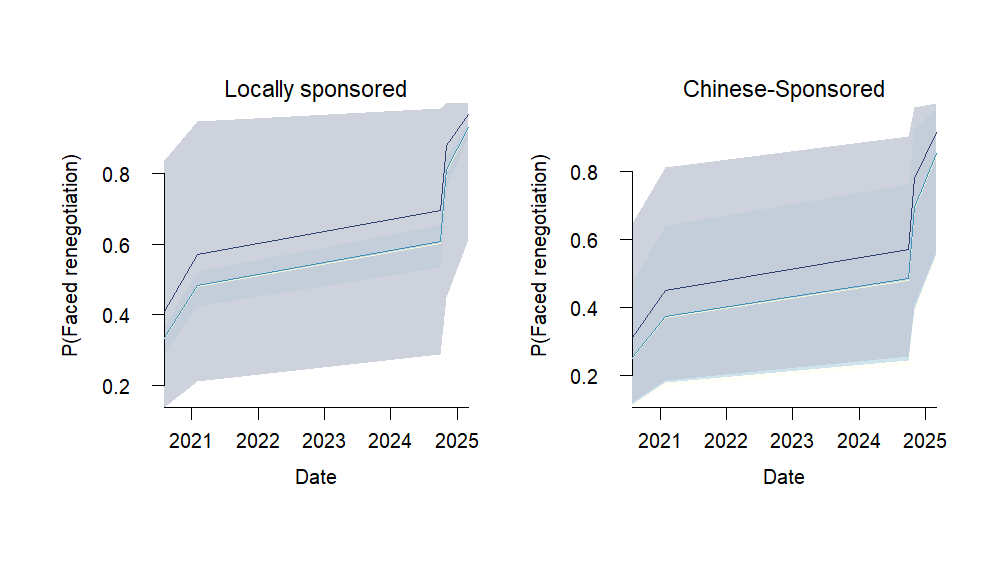
\includegraphics[width=1\linewidth]{CSSS510Final_PP.png}
    \caption{Caption}
    \label{fig:placeholder}
\end{figure}

Taken together, the results provide inconclusive evidence for the core theoretical claim: Chinese-backed IPPs are systematically insulated from renegotiation efforts.

\section{Conclusion}
We plan to implement the rest of our planned data collection and therefore run our complete suite of models. Moreover, we plan to implement log-transformed capacity and revenue, which should significantly improve our estimator's confidence interval.

Pakistan’s energy sector crisis is not merely a result of flawed contracts or poor economic planning; it is the outcome of a vertically integrated political economy. The theory of Vertical Political Integration explains how states with weak institutions and chronic instability can nonetheless sustain long-term investment relationships through selective property rights enforcement, rent-sharing, and informal sanction mechanisms. In the case of Pakistan’s IPP agreements under CPEC, the VPI coalition involves the Pakistani government, Chinese IPPs, and the Chinese state acting as a third-party enforcer. This coalition has proven remarkably resilient---weathering electoral changes, IMF bailouts, and mass public protests.

Understanding the VPI structure helps move beyond simplistic diagnoses of corruption or incompetence. It reveals the underlying logic of coalition politics, strategic dependency, and international entrenchment that shape investment flows in fragile states. Reform, if possible, will require either a shift in the coalition structure, such as the emergence of new political alignments capable of reconfiguring the rent-sharing equilibrium.

\bibliographystyle{apalike}
\bibliography{references}

\end{document}
